\documentclass{standalone}
\usepackage{tikz}
\usetikzlibrary{patterns, positioning}
\usepackage[sfdefault]{ClearSans} %% option 'sfdefault' activates Clear Sans as the default text font
\usepackage[T1]{fontenc}

\begin{document}
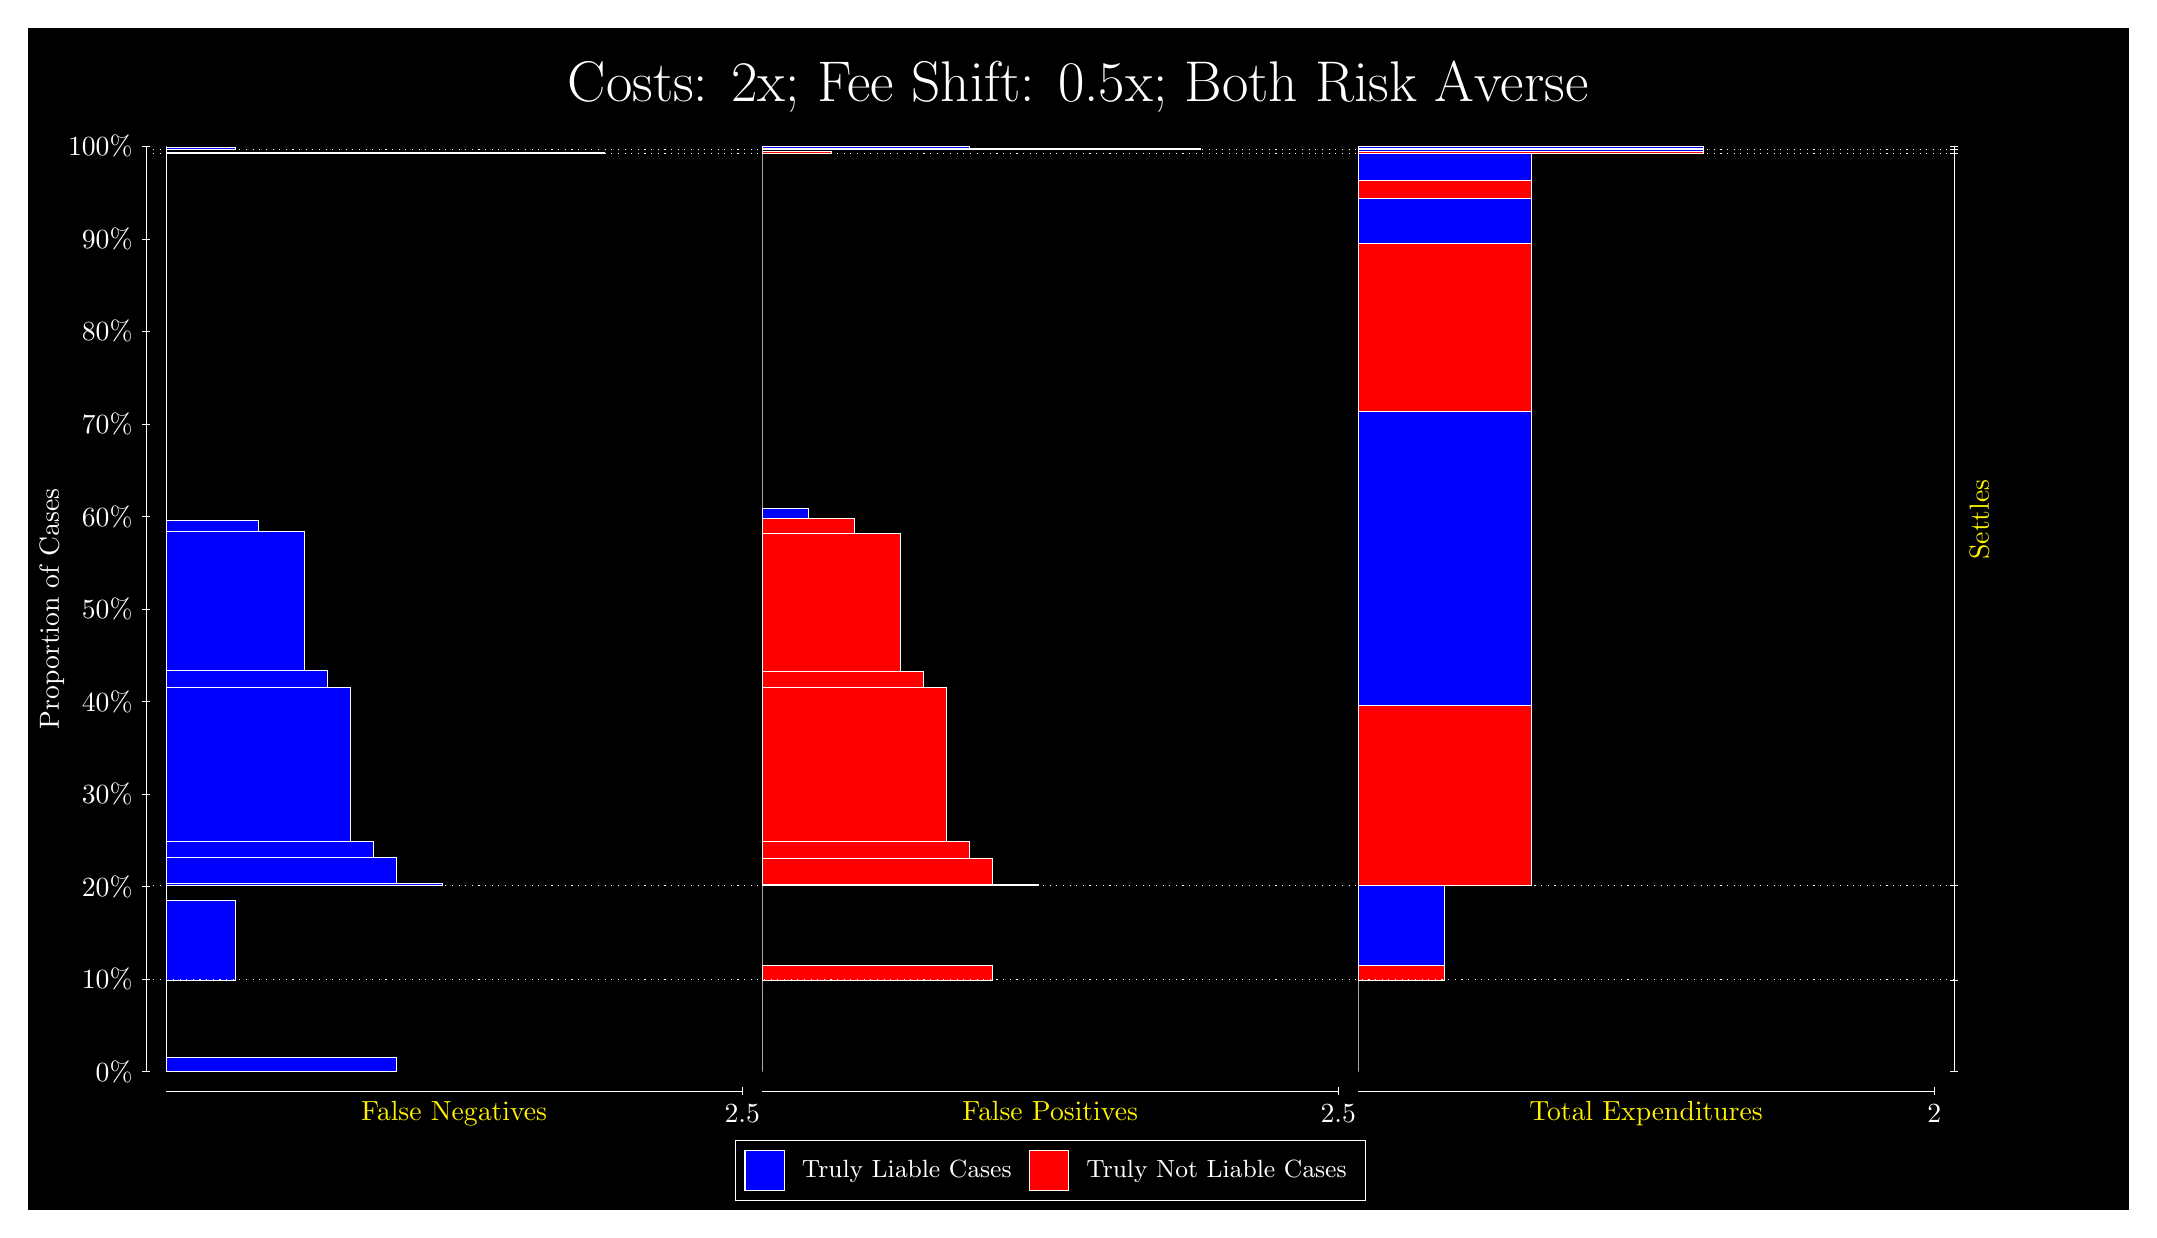
\begin{tikzpicture}
\draw[fill=black] (0,0) rectangle (26.667,15);
\draw[text=white] (0,13.5) rectangle (26.667,15) node[midway] {\huge Costs: 2x; Fee Shift: 0.5x; Both Risk Averse};
\draw[white, very thin] (1.5,1.75) -- (1.5,13.5);
\node[rotate=90, text=white, anchor=center] at (0.3, 7.625) {Proportion of Cases};
\draw[white, very thin] (1.45,1.75) -- (1.55,1.75);
\node[text=white, anchor=east] at (1.45, 1.75) {0\%};
\draw[white, very thin] (1.45,2.925) -- (1.55,2.925);
\node[text=white, anchor=east] at (1.45, 2.925) {10\%};
\draw[white, very thin] (1.45,4.1) -- (1.55,4.1);
\node[text=white, anchor=east] at (1.45, 4.1) {20\%};
\draw[white, very thin] (1.45,5.275) -- (1.55,5.275);
\node[text=white, anchor=east] at (1.45, 5.275) {30\%};
\draw[white, very thin] (1.45,6.45) -- (1.55,6.45);
\node[text=white, anchor=east] at (1.45, 6.45) {40\%};
\draw[white, very thin] (1.45,7.625) -- (1.55,7.625);
\node[text=white, anchor=east] at (1.45, 7.625) {50\%};
\draw[white, very thin] (1.45,8.8) -- (1.55,8.8);
\node[text=white, anchor=east] at (1.45, 8.8) {60\%};
\draw[white, very thin] (1.45,9.975) -- (1.55,9.975);
\node[text=white, anchor=east] at (1.45, 9.975) {70\%};
\draw[white, very thin] (1.45,11.15) -- (1.55,11.15);
\node[text=white, anchor=east] at (1.45, 11.15) {80\%};
\draw[white, very thin] (1.45,12.325) -- (1.55,12.325);
\node[text=white, anchor=east] at (1.45, 12.325) {90\%};
\draw[white, very thin] (1.45,13.5) -- (1.55,13.5);
\node[text=white, anchor=east] at (1.45, 13.5) {100\%};

\draw[white, very thin] (24.457,1.75) -- (24.457,13.5);
\draw[white, very thin] (24.407,1.75) -- (24.507,1.75);
\node[anchor=west] at (24.407, 1.75) {};
\draw[white, very thin] (24.407,2.9151) -- (24.507,2.9151);
\node[anchor=west] at (24.407, 2.9151) {};
\draw[white, very thin] (24.407,4.1109) -- (24.507,4.1109);
\node[anchor=west] at (24.407, 4.1109) {};
\draw[white, very thin] (24.407,13.412) -- (24.507,13.412);
\node[anchor=west] at (24.407, 13.412) {};
\draw[white, very thin] (24.407,13.457) -- (24.507,13.457);
\node[anchor=west] at (24.407, 13.457) {};
\draw[white, very thin] (24.407,13.5) -- (24.507,13.5);
\node[anchor=west] at (24.407, 13.5) {};

\draw[white, very thin, fill=blue] (1.75,1.75) rectangle (4.6775,1.9274);
\draw[white, very thin, fill=red] (1.75,1.9274) rectangle (1.75,2.9151);
\draw[white, very thin, fill=blue] (1.75,2.9151) rectangle (2.6283,3.9311);
\draw[white, very thin, fill=red] (1.75,3.9311) rectangle (1.75,4.1109);
\draw[white, very thin, fill=blue] (1.75,4.1109) rectangle (5.2631,4.1395);
\draw[white, very thin, fill=blue] (1.75,4.1395) rectangle (4.6775,4.4665);
\draw[white, very thin, fill=blue] (1.75,4.4665) rectangle (4.3848,4.6759);
\draw[white, very thin, fill=blue] (1.75,4.6759) rectangle (4.092,6.6325);
\draw[white, very thin, fill=blue] (1.75,6.6325) rectangle (3.7993,6.8407);
\draw[white, very thin, fill=blue] (1.75,6.8407) rectangle (3.5065,8.614);
\draw[white, very thin, fill=blue] (1.75,8.614) rectangle (2.921,8.7491);
\draw[white, very thin, fill=red] (1.75,8.7491) rectangle (1.75,13.412);
\draw[white, very thin, fill=blue] (1.75,13.412) rectangle (7.3123,13.426);
\draw[white, very thin, fill=red] (1.75,13.426) rectangle (1.75,13.457);
\draw[white, very thin, fill=blue] (1.75,13.457) rectangle (2.6283,13.485);
\draw[white, very thin, fill=red] (1.75,13.485) rectangle (1.75,13.5);
\draw[white, very thin, fill=red] (9.3189,1.75) rectangle (9.3189,2.7378);
\draw[white, very thin, fill=blue] (9.3189,2.7378) rectangle (9.3189,2.9151);
\draw[white, very thin, fill=red] (9.3189,2.9151) rectangle (12.246,3.0949);
\draw[white, very thin, fill=blue] (9.3189,3.0949) rectangle (9.3189,4.1109);
\draw[white, very thin, fill=red] (9.3189,4.1109) rectangle (12.832,4.1323);
\draw[white, very thin, fill=red] (9.3189,4.1323) rectangle (12.246,4.4623);
\draw[white, very thin, fill=red] (9.3189,4.4623) rectangle (11.954,4.6718);
\draw[white, very thin, fill=red] (9.3189,4.6718) rectangle (11.661,6.6305);
\draw[white, very thin, fill=red] (9.3189,6.6305) rectangle (11.368,6.8387);
\draw[white, very thin, fill=red] (9.3189,6.8387) rectangle (11.075,8.5861);
\draw[white, very thin, fill=red] (9.3189,8.5861) rectangle (10.49,8.7733);
\draw[white, very thin, fill=blue] (9.3189,8.7733) rectangle (9.9044,8.9085);
\draw[white, very thin, fill=blue] (9.3189,8.9085) rectangle (9.3189,13.412);
\draw[white, very thin, fill=red] (9.3189,13.412) rectangle (10.197,13.442);
\draw[white, very thin, fill=blue] (9.3189,13.442) rectangle (9.3189,13.457);
\draw[white, very thin, fill=red] (9.3189,13.457) rectangle (14.881,13.471);
\draw[white, very thin, fill=blue] (9.3189,13.471) rectangle (11.954,13.5);
\draw[white, very thin, fill=red] (16.888,1.75) rectangle (16.888,2.7378);
\draw[white, very thin, fill=blue] (16.888,2.7378) rectangle (16.888,2.9151);
\draw[white, very thin, fill=red] (16.888,2.9151) rectangle (17.986,3.0949);
\draw[white, very thin, fill=blue] (16.888,3.0949) rectangle (17.986,4.1109);
\draw[white, very thin, fill=red] (16.888,4.1109) rectangle (19.083,6.3996);
\draw[white, very thin, fill=blue] (16.888,6.3996) rectangle (19.083,10.129);
\draw[white, very thin, fill=red] (16.888,10.129) rectangle (19.083,12.272);
\draw[white, very thin, fill=blue] (16.888,12.272) rectangle (19.083,12.837);
\draw[white, very thin, fill=red] (16.888,12.837) rectangle (19.083,13.068);
\draw[white, very thin, fill=blue] (16.888,13.068) rectangle (19.083,13.412);
\draw[white, very thin, fill=red] (16.888,13.412) rectangle (21.279,13.442);
\draw[white, very thin, fill=blue] (16.888,13.442) rectangle (21.279,13.457);
\draw[white, very thin, fill=red] (16.888,13.457) rectangle (21.279,13.471);
\draw[white, very thin, fill=blue] (16.888,13.471) rectangle (21.279,13.5);
\draw[white, dotted] (1.5,2.9151) -- (24.457,2.9151);
\draw[white, dotted] (1.5,4.1109) -- (24.457,4.1109);
\draw[white, dotted] (1.5,13.412) -- (24.457,13.412);
\draw[white, dotted] (1.5,13.457) -- (24.457,13.457);
\draw[white, very thin] (1.75,1.5) -- (9.0689,1.5);
\node[text=yellow, anchor=north] at (5.4094, 1.5) {False Negatives};
\draw[white, very thin] (9.0689,1.45) -- (9.0689,1.55);
\node[text=white, anchor=north] at (9.0689, 1.45) {2.5};

\draw[white, very thin] (9.3189,1.5) -- (16.638,1.5);
\node[text=yellow, anchor=north] at (12.978, 1.5) {False Positives};
\draw[white, very thin] (16.638,1.45) -- (16.638,1.55);
\node[text=white, anchor=north] at (16.638, 1.45) {2.5};

\draw[white, very thin] (16.888,1.5) -- (24.207,1.5);
\node[text=yellow, anchor=north] at (20.547, 1.5) {Total Expenditures};
\draw[white, very thin] (24.207,1.45) -- (24.207,1.55);
\node[text=white, anchor=north] at (24.207, 1.45) {2};



\node[text=yellow, centered, rotate=90] at (24.777, 8.7612) {Settles};



\draw (12.978300999999998,1.5) node[draw=none] (baseCoordinate) {};
\begin{scope}[align=center]
        \matrix[scale=0.5, draw=white, below=0.5cm of baseCoordinate, nodes={draw}, column sep=0.1cm]{
            \node[rectangle, draw, minimum width=0.5cm, minimum height=0.5cm, fill=blue] {}; &
            \node[draw=none, font=\small, text=white] (B) {Truly Liable Cases}; &
            \node[rectangle, draw, minimum width=0.5cm, minimum height=0.5cm, fill=red] {}; &
            \node[draw=none, font=\small, text=white] (B) {Truly Not Liable Cases}; \\
            };
\end{scope}

\end{tikzpicture}
\end{document}